
\documentclass[a4paper,11pt]{article}
\usepackage[a4paper, margin=8em]{geometry}

% usa i pacchetti per la scrittura in italiano
\usepackage[french,italian]{babel}
\usepackage[T1]{fontenc}
\usepackage[utf8]{inputenc}
\frenchspacing 

% usa i pacchetti per la formattazione matematica
\usepackage{amsmath, amssymb, amsthm, amsfonts}

% usa altri pacchetti
\usepackage{gensymb}
\usepackage{hyperref}
\usepackage{standalone}

\usepackage{colortbl}

\usepackage{xstring}
\usepackage{karnaugh-map}

% imposta il titolo
\title{Appunti Calcolatori Elettronici}
\author{Luca Seggiani}
\date{2025}

% imposta lo stile
% usa helvetica
\usepackage[scaled]{helvet}
% usa palatino
\usepackage{palatino}
% usa un font monospazio guardabile
\usepackage{lmodern}

\renewcommand{\rmdefault}{ppl}
\renewcommand{\sfdefault}{phv}
\renewcommand{\ttdefault}{lmtt}

% circuiti
\usepackage{circuitikz}
\usetikzlibrary{babel}

% testo cerchiato
\newcommand*\circled[1]{\tikz[baseline=(char.base)]{
            \node[shape=circle,draw,inner sep=2pt] (char) {#1};}}

% disponi il titolo
\makeatletter
\renewcommand{\maketitle} {
	\begin{center} 
		\begin{minipage}[t]{.8\textwidth}
			\textsf{\huge\bfseries \@title} 
		\end{minipage}%
		\begin{minipage}[t]{.2\textwidth}
			\raggedleft \vspace{-1.65em}
			\textsf{\small \@author} \vfill
			\textsf{\small \@date}
		\end{minipage}
		\par
	\end{center}

	\thispagestyle{empty}
	\pagestyle{fancy}
}
\makeatother

% disponi teoremi
\usepackage{tcolorbox}
\newtcolorbox[auto counter, number within=section]{theorem}[2][]{%
	colback=blue!10, 
	colframe=blue!40!black, 
	sharp corners=northwest,
	fonttitle=\sffamily\bfseries, 
	title=Teorema~\thetcbcounter: #2, 
	#1
}

% disponi definizioni
\newtcolorbox[auto counter, number within=section]{definition}[2][]{%
	colback=red!10,
	colframe=red!40!black,
	sharp corners=northwest,
	fonttitle=\sffamily\bfseries,
	title=Definizione~\thetcbcounter: #2,
	#1
}

% disponi codice
\usepackage{listings}
\usepackage[table]{xcolor}

\definecolor{codegreen}{rgb}{0,0.6,0}
\definecolor{codegray}{rgb}{0.5,0.5,0.5}
\definecolor{codepurple}{rgb}{0.58,0,0.82}
\definecolor{backcolour}{rgb}{0.95,0.95,0.92}

\lstdefinestyle{codestyle}{
		backgroundcolor=\color{black!5}, 
		commentstyle=\color{codegreen},
		keywordstyle=\bfseries\color{magenta},
		numberstyle=\sffamily\tiny\color{black!60},
		stringstyle=\color{green!50!black},
		basicstyle=\ttfamily\footnotesize,
		breakatwhitespace=false,         
		breaklines=true,                 
		captionpos=b,                    
		keepspaces=true,                 
		numbers=left,                    
		numbersep=5pt,                  
		showspaces=false,                
		showstringspaces=false,
		showtabs=false,                  
		tabsize=2
}

\lstdefinestyle{shellstyle}{
		backgroundcolor=\color{black!5}, 
		basicstyle=\ttfamily\footnotesize\color{black}, 
		commentstyle=\color{black}, 
		keywordstyle=\color{black},
		numberstyle=\color{black!5},
		stringstyle=\color{black}, 
		showspaces=false,
		showstringspaces=false, 
		showtabs=false, 
		tabsize=2, 
		numbers=none, 
		breaklines=true
}


\lstdefinelanguage{assembler}{ 
  keywords={AAA, AAD, AAM, AAS, ADC, ADCB, ADCW, ADCL, ADD, ADDB, ADDW, ADDL, AND, ANDB, ANDW, ANDL,
        ARPL, BOUND, BSF, BSFL, BSFW, BSR, BSRL, BSRW, BSWAP, BT, BTC, BTCB, BTCW, BTCL, BTR, 
        BTRB, BTRW, BTRL, BTS, BTSB, BTSW, BTSL, CALL, CBW, CDQ, CLC, CLD, CLI, CLTS, CMC, CMP,
        CMPB, CMPW, CMPL, CMPS, CMPSB, CMPSD, CMPSW, CMPXCHG, CMPXCHGB, CMPXCHGW, CMPXCHGL,
        CMPXCHG8B, CPUID, CWDE, DAA, DAS, DEC, DECB, DECW, DECL, DIV, DIVB, DIVW, DIVL, ENTER,
        HLT, IDIV, IDIVB, IDIVW, IDIVL, IMUL, IMULB, IMULW, IMULL, IN, INB, INW, INL, INC, INCB,
        INCW, INCL, INS, INSB, INSD, INSW, INT, INT3, INTO, INVD, INVLPG, IRET, IRETD, JA, JAE,
        JB, JBE, JC, JCXZ, JE, JECXZ, JG, JGE, JL, JLE, JMP, JNA, JNAE, JNB, JNBE, JNC, JNE, JNG,
        JNGE, JNL, JNLE, JNO, JNP, JNS, JNZ, JO, JP, JPE, JPO, JS, JZ, LAHF, LAR, LCALL, LDS,
        LEA, LEAVE, LES, LFS, LGDT, LGS, LIDT, LMSW, LOCK, LODSB, LODSD, LODSW, LOOP, LOOPE,
        LOOPNE, LSL, LSS, LTR, MOV, MOVB, MOVW, MOVL, MOVSB, MOVSD, MOVSW, MOVSX, MOVSXB,
        MOVSXW, MOVSXL, MOVZX, MOVZXB, MOVZXW, MOVZXL, MUL, MULB, MULW, MULL, NEG, NEGB, NEGW,
        NEGL, NOP, NOT, NOTB, NOTW, NOTL, OR, ORB, ORW, ORL, OUT, OUTB, OUTW, OUTL, OUTSB, OUTSD,
        OUTSW, POP, POPL, POPW, POPB, POPA, POPAD, POPF, POPFD, PUSH, PUSHL, PUSHW, PUSHB, PUSHA, 
				PUSHAD, PUSHF, PUSHFD, RCL, RCLB, RCLW, MOVSL, MOVSB, MOVSW, STOSL, STOSB, STOSW, LODSB, LODSW,
				LODSL, INSB, INSW, INSL, OUTSB, OUTSL, OUTSW
        RCLL, RCR, RCRB, RCRW, RCRL, RDMSR, RDPMC, RDTSC, REP, REPE, REPNE, RET, ROL, ROLB, ROLW,
        ROLL, ROR, RORB, RORW, RORL, SAHF, SAL, SALB, SALW, SALL, SAR, SARB, SARW, SARL, SBB,
        SBBB, SBBW, SBBL, SCASB, SCASD, SCASW, SETA, SETAE, SETB, SETBE, SETC, SETE, SETG, SETGE,
        SETL, SETLE, SETNA, SETNAE, SETNB, SETNBE, SETNC, SETNE, SETNG, SETNGE, SETNL, SETNLE,
        SETNO, SETNP, SETNS, SETNZ, SETO, SETP, SETPE, SETPO, SETS, SETZ, SGDT, SHL, SHLB, SHLW,
        SHLL, SHLD, SHR, SHRB, SHRW, SHRL, SHRD, SIDT, SLDT, SMSW, STC, STD, STI, STOSB, STOSD,
        STOSW, STR, SUB, SUBB, SUBW, SUBL, TEST, TESTB, TESTW, TESTL, VERR, VERW, WAIT, WBINVD,
        XADD, XADDB, XADDW, XADDL, XCHG, XCHGB, XCHGW, XCHGL, XLAT, XLATB, XOR, XORB, XORW, XORL},
  keywordstyle=\color{blue}\bfseries,
  ndkeywordstyle=\color{darkgray}\bfseries,
  identifierstyle=\color{black},
  sensitive=false,
  comment=[l]{\#},
  morecomment=[s]{/*}{*/},
  commentstyle=\color{purple}\ttfamily,
  stringstyle=\color{red}\ttfamily,
  morestring=[b]',
  morestring=[b]"
}

\lstset{language=assembler, style=codestyle}

% disponi sezioni
\usepackage{titlesec}

\titleformat{\section}
	{\sffamily\Large\bfseries} 
	{\thesection}{1em}{} 
\titleformat{\subsection}
	{\sffamily\large\bfseries}   
	{\thesubsection}{1em}{} 
\titleformat{\subsubsection}
	{\sffamily\normalsize\bfseries} 
	{\thesubsubsection}{1em}{}

% tikz
\usepackage{tikz}

% float
\usepackage{float}

% grafici
\usepackage{pgfplots}
\pgfplotsset{width=10cm,compat=1.9}

% disponi alberi
\usepackage{forest}

\forestset{
	rectstyle/.style={
		for tree={rectangle,draw,font=\large\sffamily}
	},
	roundstyle/.style={
		for tree={circle,draw,font=\large}
	}
}

% disponi algoritmi
\usepackage{algorithm}
\usepackage{algorithmic}
\makeatletter
\renewcommand{\ALG@name}{Algoritmo}
\makeatother

% disponi numeri di pagina
\usepackage{fancyhdr}
\fancyhf{} 
\fancyfoot[L]{\sffamily{\thepage}}

\makeatletter
\fancyhead[L]{\raisebox{1ex}[0pt][0pt]{\sffamily{\@title \ \@date}}} 
\fancyhead[R]{\raisebox{1ex}[0pt][0pt]{\sffamily{\@author}}}
\makeatother

\begin{document}
% sezione (data)
\section{Lezione del 31-03-25}

% stili pagina
\thispagestyle{empty}
\pagestyle{fancy}

% testo
Continuiamo il discorso sulla paginazione.

\subsubsection{Funzionamento della MMU}
Avevamo definito una MMU che definiva tabelle di corrispodenza fra pagine e frame, una per ogni processo in esecuzione.
Avevamo quindi detto che il processo (diciamo $P_1$) in esecuzione ha più sezioni di dati, cui potremmo assegnare ad esempio un frame ciascuna:
\begin{table}[H]
	\center
	\begin{tabular} { | c | c | }
		\bfseries Sezione & \bfseries Frame \\
		\hline
		\textsf{Text (Code)} $P_1$ & 2 \\
		\textsf{Data} $P_1$ & 3 \\
		... & // \\
		\textsf{Stack} $P_1$ & 4 \\
	\end{tabular}
\end{table}

I \textit{frame} di memoria scelti e sono in posizioni arbitrarie, l'unica cosa importante è che la MMU li possa rintracciare attraverso le sue tabelle di corrispondenza.

Potremo quindi assumere che la pagina 0 sia riservata, la pagina 1 riservata al sistema, e vedere che una tabella di corrispondenza per $P_1$ potrebbe essere la seguente:
\begin{table}[H]
	\center
	\begin{tabular} { | c | c | c | }
		\bfseries Pagina & \bfseries Sezione & \bfseries Frame \\
		\hline
		0 & \textsf{Null} & // \\
		1 & \textsf{Sistema} & 1 \\
		2 & \textsf{Text} $P_1$ & 2 \\
		3 & \textsf{Data} $P_1$ & 3 \\
		... & ... & // \\
		7 & \textsf{Stack} $P_1$ & 4 \\
	\end{tabular}
\end{table}
dove si è scelto di disporre lo stack in fondo allo spazio di memoria.

Nel momento in cui un altro processo (diciamo $P_2$) entra in esecuzione, potremmo assegnargli le seguenti pagine:
\begin{table}[H]
	\center
	\begin{tabular} { | c | c | }
		\bfseries Sezione & \bfseries Frame \\
		\hline
		\textsf{Text} $P_2$ & 5 \\
		\textsf{Data} $P_2$ & 6 \\
		... & // \\
		\textsf{Stack} $P_2$ & 7 \\
	\end{tabular}
\end{table}
e disporre una tabella di corrispondenza:
\begin{table}[H]
	\center
	\begin{tabular} { | c | c | c | }
		\bfseries Pagina & \bfseries Sezione & \bfseries Frame \\
		\hline
		0 & \textsf{Null} & 0 \\
		1 & \textsf{Sistema} & 1 \\
		2 & \textsf{Text} $P_2$ & 5 \\
		3 & \textsf{Data} $P_2$ & 6 \\
		... &... & // \\
		7 & \textsf{Stack} $P_2$ & 7 \\
	\end{tabular}
\end{table}

Vediamo che la pagina sistema resta nella tabella, ergo quella pagina è \textbf{condivisa} fra più processi.
Cambiare contesto significherà quindi, oltre che caricare i registri, passare da una tabella di corrispondenza di processo all'altra.
Il fatto che la pagina sistema sia sempre la 1 ci assicura che i suoi indirizzi siano per il programmatore sempre gli stessi.

\subsubsection{Verso la MMU reale}
Vediamo che la MMU come l'abbiamo definita adesso è effettivamente di impossibile realizzazione.
Vediamo infatti le dimensione di queste tabelle: se si prendono 12 bit di offset, per pagine da 4 KiB, si ha che nei 48 bit indirizzabili dall'architettura x86 (senza estendere a 57) lasciano 36 bit, e quindi $2^{36}$, cioè 64 miliardi (64 Gi, \textit{Gibi}) circa di pagine.
Se vogliamo dedicare 8 byte ad ogni entrata di una tabella di corrispondenza, quindi, abbiamo bisogno di 512 GiB di spazio, che non è chiaramente fattibile (considerando poi che vogliamo una tabella per processo, quindi moltiplicando questo valore per un $n$ arbitrariamente grande).

Chiamiamo quindi il modello fittizio visto finora \textbf{S-MMU} (da \textit{Super MMU}) e ne introduciamo una versione più vicina alla realtà, che adotta una struttura dati diversa: la \textbf{T-MMU} (da \textit{Trie MMU}).

La \textbf{trie} è una struttura dati che nasce per effettuare ricerche chiave-valore.
Sono simili agli alberi binari, con la differenza che la chiave non è memorizzata nei nodi, ma nella posizione stessa dei nodi all'interno dell'albero.

Utilizziamo le trie per realizzare una struttura dati detta \textbf{bitwise tree}, o \textit{albero bitwise}.
L'idea è quella di dividere i 36 bit di pagina in 4 porzioni da 9 bit ciascuna, sulle quali costruire delle trie.
La radice della struttura che costruiamo sarà quindi una tabella di $2^9 = 512$ entrate, corrispondente alle 512 possibili configurazioni dei primi 9 dei 36 bit di pagina.
Ognuna di queste entrate punterà ad un altra tabella di $512$ entrate, relative ai 9 bit successivi.
Si hanno quindi 4 livelli di accesso, ordinati dal 4 all'1, che bisogna attraversare per arrivare fino al frame corrispondente alla pagina che ci interessa:

\begin{center}
	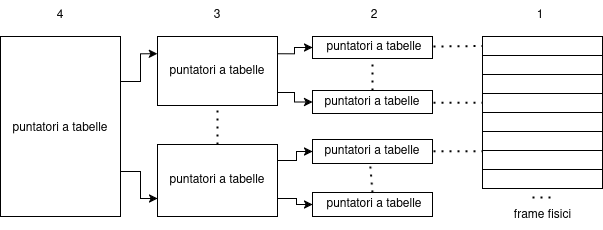
\includegraphics[scale=0.6]{../figures/mmu_trie.png}
\end{center}

Nei sistemi operativi moderni, quali Linux, ogni livello di accesso ha un nome specifico e quindi ogni segmento da 9 bit dei 36 bit di pagina rappresenta un informazione denominata diversamente, che riportiamo per completezza (dal più significativo):

\begin{table}[h!]
	\center \rowcolors{2}{white}{black!10}
	\begin{tabular} { c | c | p{7cm} }
		\bfseries Bit & \bfseries Nome & \bfseries Significato \\ 
		\hline
		9 bit & PML4I & \textit{Page Map Level 4 Index} \\
		9 bit & PDPTI & \textit{Page Directory Pointer Table Index} \\
		9 bit & PDI & \textit{Page Directory Index} \\
		9 bit & PTI & \textit{Page Table Index} \\
		12 bit & // & Offset di pagina 
	\end{tabular}
\end{table}

Resta comunque il fatto che quale nome decidiamo di assegnare alle tabelle di ogni livello di accesso non è importante, in quanto le strutture ad ogni livello sono sovrapposte (puntare a una tabella o a un frame è la stessa cosa).

Il procedimento che ci porta dai bit di pagina all'indirizzo del frame si chiama \textbf{table walk}, o \textit{cammino della tabella}.
Ogni entrata delle tabelle di trie sarà grande 8 byte (almeno 7 bit per i flag, più $\sim 48$ bit di indirizzo, ricordando che lo spazio indirizzabile nell'x86\_64 non corrisponde al massimo di 64 bit), per cui $2^9 \cdot 2^3 = 2^{12} = 4\text{ KiB}$ di memoria ciascuna.

\noindent
\begin{minipage}{\textwidth}
La memoria massima \textit{raggiunta ad} ogni livello e il numero di entrate \textit{raggiunta ad} ogni livello sono quindi:

\begin{table}[H]
	\center \rowcolors{2}{white}{black!10}
	\begin{tabular} { c | p{6cm} | p{6cm} }
		\bfseries Livello & \bfseries Memoria massima usata & \bfseries Numero di entrate \\ 
		\hline 
		4 & $2^9 \cdot 2^3 = 2^{12} = 4 \text{ KiB}$                       & $2^9 = 512$ \\
		3 & $2^9 \cdot 2^9 \cdot 2^3 = 2^{21} = 2 \text{ MiB}$             & $2^9 \cdot 2^9 = 2^{18} = 256 \text{ Ki}$ \\            
		2 & $2^9 \cdot 2^9 \cdot 2^9 \cdot 2^3 = 2^{30} = 1 \text{ GiB}$   & $2^9 \cdot 2^9 \cdot 2^9 = 2^{27} = 128 \text{ Mi}$ \\ 
		1 & $2^9 \cdot 2^9 \cdot 2^9 \cdot 2^9 \cdot 2^3 = 2^{39} = 512 \text{ GiB}$ & $2^9 \cdot 2^9 \cdot 2^9 \cdot 2^9 = 2^{36} = 64 \text{ Gi}$
	\end{tabular}
\end{table}
\end{minipage}
\par\bigskip

Per cottenere l'informazione inversa, cioè la memoria massima \textit{raggiungibile da} ogni livello e il numero di entrate \textit{raggiungibili da} ogni livelo basterà invertire l'ordine verticale delle ultime 2 colonne. 

Potremmo allora chiederci dov'è il guadagno di un sistema di questo tipo, in quanto a memoria l'ultimo livello di trie necessiterà degli stessi 512 GiB, più lo spazio necessario ai livelli precedenti.
Il vantaggio sarà però quello di poter tagliare arbitrariamente rami dall'albero che abbiamo formato, cioè non tenere conto di pagine di cui non abbiamo attualmente bisogno. 

\subsubsection{Descrittori nella T-MMU}
Vediamo come si evolvono i descrittori che avevamo messa corredo delle tabelle di corrispondenza, nella T-MMU.
Avremo che ci dovrà essere una distinzione fra i descrittori di primo e di secondo, terzo e quarto livello:
\begin{itemize}
	\item \textbf{Descrittori di primo livello:}
		qui vogliamo usare l'intero insieme di descrittori, che riportiamo:
\begin{center}
	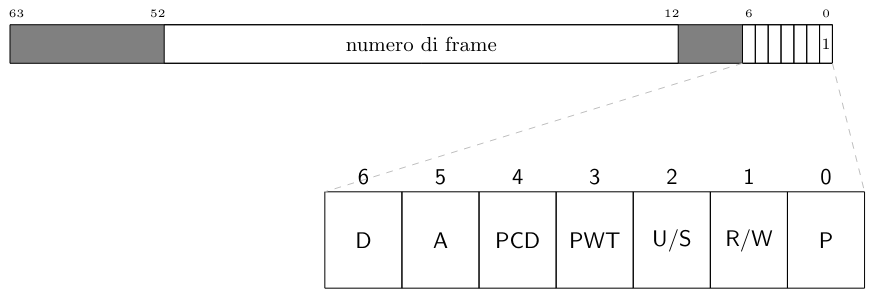
\includegraphics[scale=0.6]{../figures/mmu_level1.png}
\end{center}
\begin{itemize}
	\item \textbf{P:} un bit di presenza, che definisce l'esistenza o meno di una traduzione per quell'indirizzo: nel caso di accesso a pagine non traducibili si genera un ecceione, detta \textbf{page fault}, che comporta il caricamento della pagina richiesta o la terminazione forzata del programma per \textbf{segmentation fault}.

		Ad esempio, se scegliamo 0 come la codifica del null pointer, vogliamo che la prima pagina (o le prime pagine, se vogliamo essere più larghi con accessi a strutture puntate da null pointer, che potrebbero avere offset negli struct anche consideravoli) sia non presente, e quindi si traduca in eccezione prima di effettuare accessi chiaramente erronei;
	\item \textbf{S/U:} \textit{Sistema/Utente}, indica se una pagina è accessibile o meno ad un processo utente;  
	\item \textbf{R/W:} \textit{Read/Write}, indica se una pagina è accessibile solo in scrittura o solo in lettura per un certo processo. 
		Questa può essere utile ad esempio per la sezione \textit{text} del programma, che ricordiamo contiene il codice e non vogliamo venga modificata;
	\item \textbf{PCD} e \textbf{PWT}: indicano se ignorare completamente la cache (PCD) o se adottare una politica di scrittura \textit{write-through} (PWT).
		Questo può essere utile nel caso di dispositivi mappati in memoria (come l'APIC o l'adattatore video);
	\item \textbf{A} e \textbf{D}: due flag che danno indicazioni agli accessi che la MMU ha individuato sulla pagina.

		Vediamo solo adesso la loro utilità: la MMU setta questi bit per dare informazioni al kernel su cosa è successo alle pagine fino all'ultimo accesso.
		Il bit \textbf{A}, quindi, indica che una certa pagina è stata usata (\textit{attraversata}), mentre il bit \textbf{D} (\textit{Dirty}) indica che si è scritto su una certa pagina. 
		Abbiamo quindi una situazione dove è l'\textit{hardware} ad informare il \textit{software} del suo funzionamento, e non viceversa (come eravamo abituati). 
		L'informazione può quindi essere usata per gestire meglio il caricamento su e da memoria delle pagine, sopratutto in sistemi che supportano la \textit{memoria di swap}, cioè una certa porzione di memoria sul disco rigido che viene impiegata nella memorizzazione delle immagini dei processi in esecuzione (che è come, in origine, avevamo ipotizzato funzionasse il meccanismo della multiprogrammazione).
		In questo caso conoscere il flag D può evitare una scrittura su disco quando una pagina non è stata modificata, mentre conoscere il flag A può dare un euristica su quali pagine conviene spostare nello swap e quali mantenere nel caso di spostamento di pagine da e su disco.
		Per la precisione, in sistemi di questo tipo i pagefault sono normali, e vengono sfruttati per realizzare la \textit{paginazione su domanda}: può essere che la pagina richiesta da un processo non esista, quindi comporti un'eccezione, che viene gestita caricando la pagina corrispondente (e quindi verificando i flag A se altre pagine vanno rimosse per fare spazio).
\end{itemize}

	\item \textbf{Descrittori di secondo, terzo e quarto livello:} il descrittore ha questo aspetto:
\begin{center}
	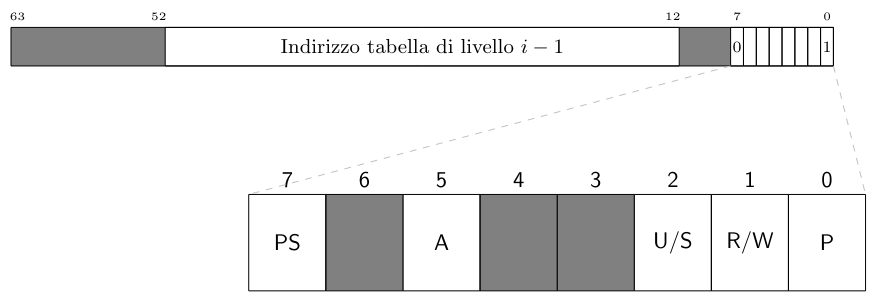
\includegraphics[scale=0.6]{../figures/mmu_level234.png}
\end{center}
		in questo caso non abbiamo bisogno di \textbf{PWT}, \textbf{PCT} e \textbf{D}, mentre introduciamo un nuovo bit, \textbf{PS}, \textit{Page Size}, che distingue due situazioni: se PS è basso, si procede come si è detto finora, altrimenti, quella entrata punta ad un unica pagina contigua di entrate (e non al livello successivo della trie).
		Il numero di entrate delle pagine contigue, dette \textbf{huge page}, cambia quindi in base al livello:
\begin{table}[H]
	\center \rowcolors{2}{white}{black!10}
	\begin{tabular} { c | p{6cm} }
		\bfseries Livello & \bfseries Memoria indirizzata in huge page\\ 
		\hline 
		4 & // \\ 
		3 & 1 GiB \\ 
		2 & 2 MiB \\ 
		1 & 4 Kib (default) \\
	\end{tabular}
\end{table}
in quanto, ad ogni livello, stiamo effettivamente "passando" 9 bit dall'indirizzo di pagina all'offset nella pagina, cioè stiamo adottando indirizzi e offset di dimensione:
\begin{table}[H]
	\center \rowcolors{2}{white}{black!10}
	\begin{tabular} { c | p{5cm} | p{5cm} }
		\bfseries Livello & \bfseries Dimensione indirizzo & \bfseries Dimensione offset \\ 
		\hline 
		4 & // & // \\ 
		3 & 18 bit & 30  bit \\
		2 & 27 bit & 21 bit \\ 
		1 & 36 bit & 12 bit \\
	\end{tabular}
\end{table}

Come si vede poi dalla tabella, il flag PS è effettivamente ignorato al livello 4 (avremmo pagine da 512 GB, che ad oggi non tornano particolarmente utili) e al livello 1 (è la dimensione di default delle pagine).
\end{itemize}

\subsubsection{T-MMU e memoria condivisa}
La struttura ad albero delle trie ci permette, ad esempio, di far puntare un entrata di un sottoalbero della trie associata ad un processo, ad un sottoalbero di una trie di un altro processo.
Questo ci permette effettivamente di realizzare pagine, o tabelle di pagine, condivise fra processi.
Potremo liberamente assegnare la stessa pagina in posizioni diverse dello spazio di memoria di ogni processo, in quanto l'unica cosa importante è il \textit{percorso} che ci porta alla tabella condivisa, che può variare di processo in processo (o meglio di trie di processo in trie di processo).

\end{document}
